\section{Results}

We have two goals in our case studies. First, we want to determine if there is any correlation between weather and mood. Second, we would like to verify if our predicted mood is correct.

%\begin{figure*}[htp]
%  \centering
%  \subfigure[Temperatures in Omaha and Lincoln]{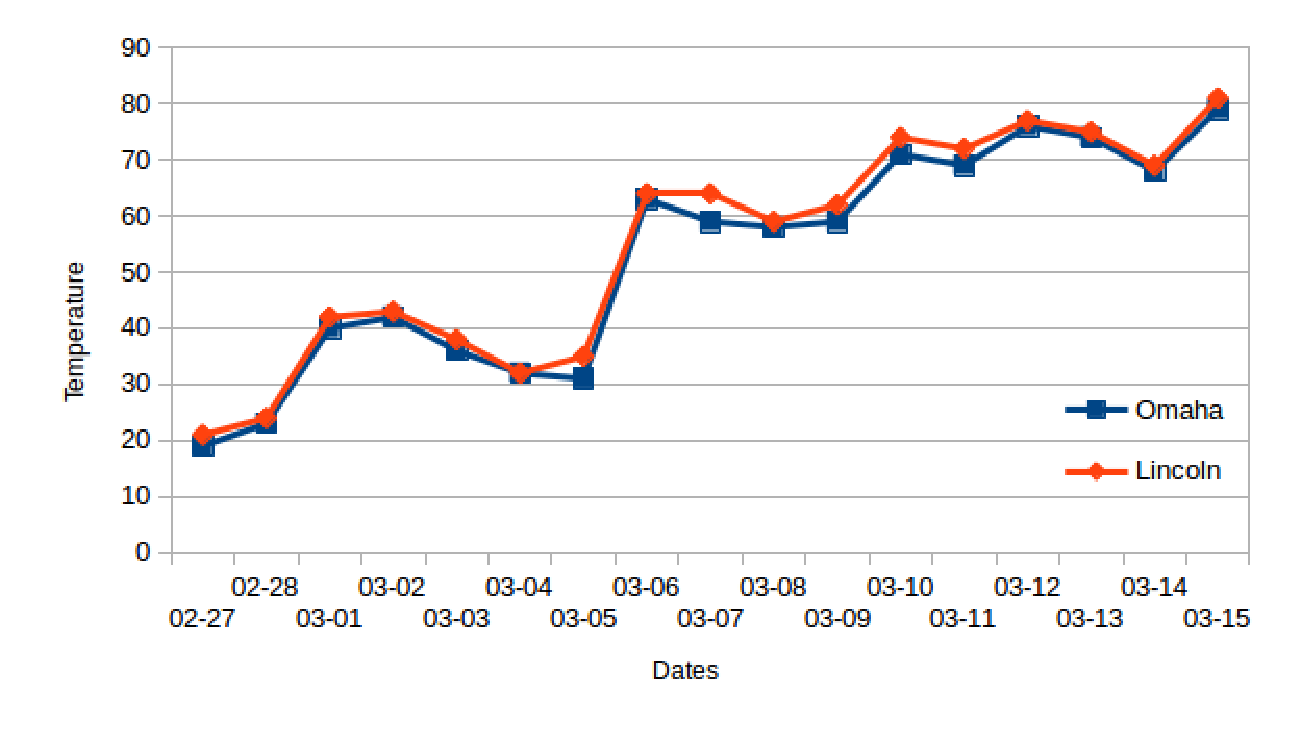
\includegraphics[scale=0.25]{chart1}}\quad
%  \subfigure[Sentiment of Omaha and Lincoln Tweets]{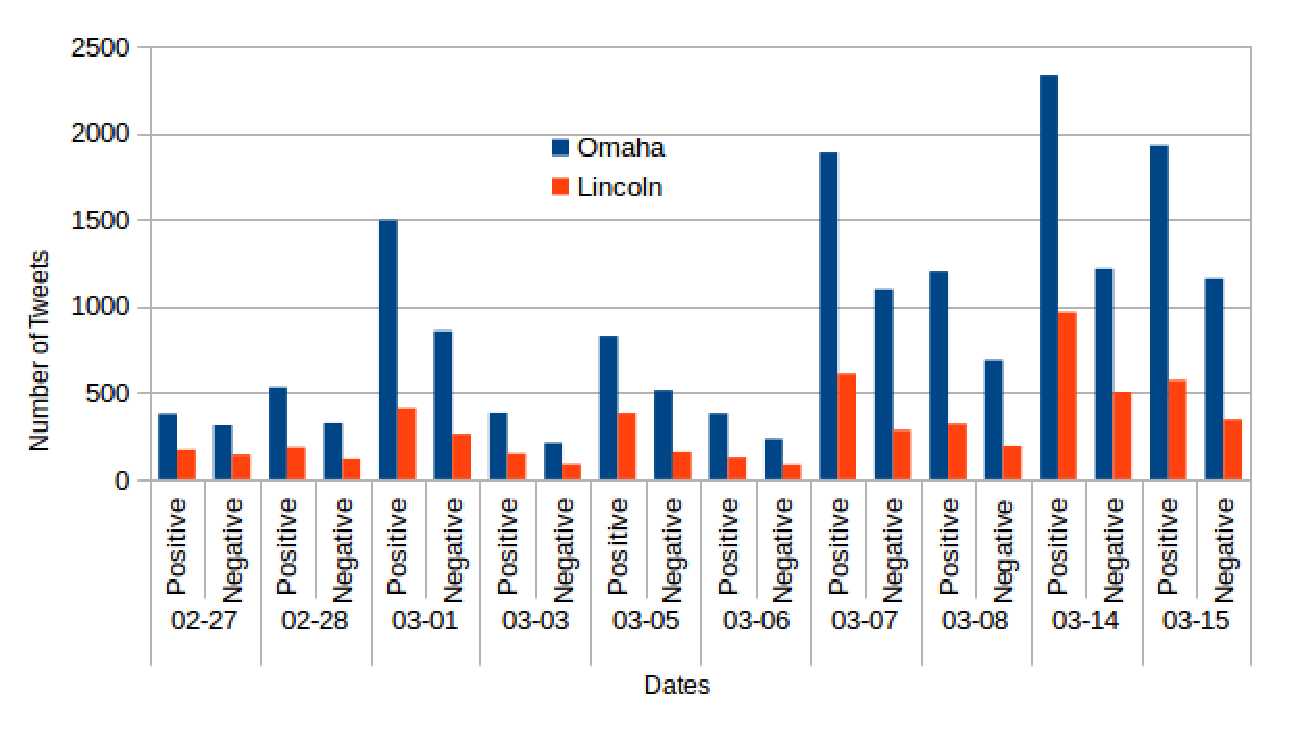
\includegraphics[scale=0.25]{chart2}}\quad
%  \subfigure[Sentiment of Omaha and Lincoln Tweets]{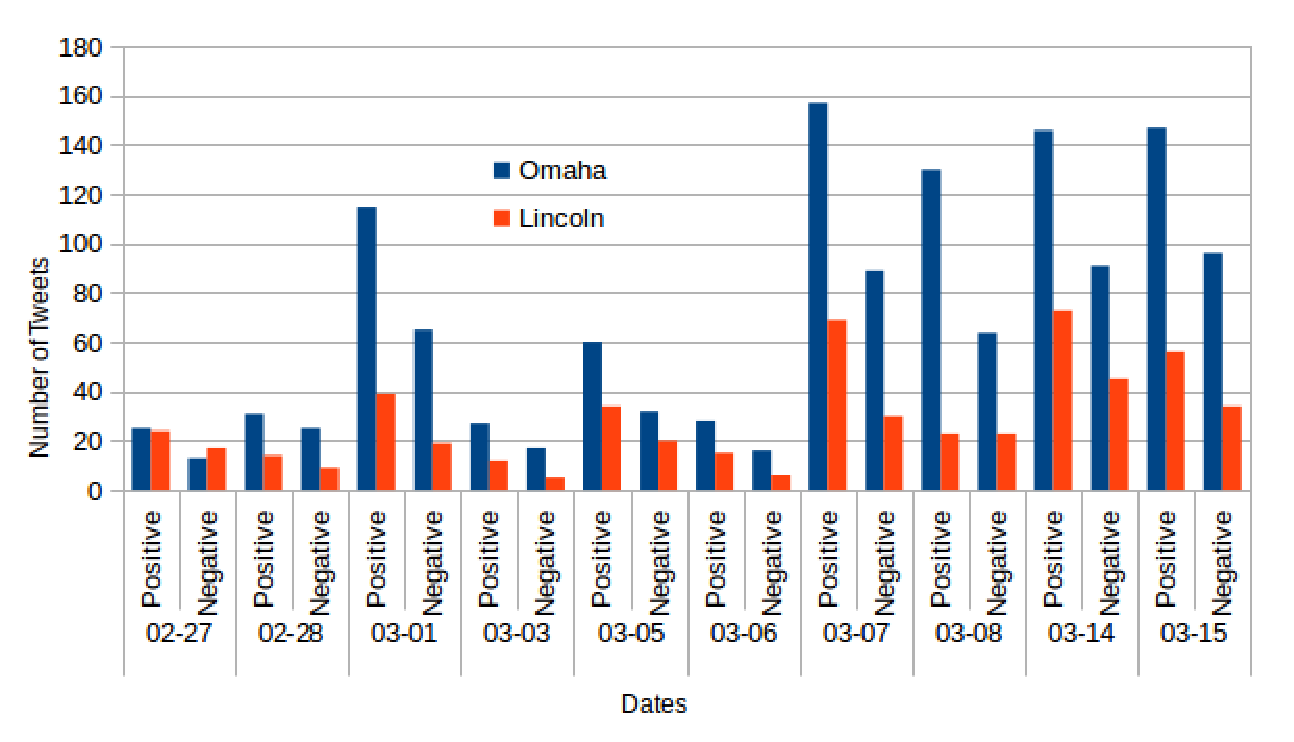
\includegraphics[scale=0.25]{chart3}}
%\caption{The comparison of weather to sentiment.}
%\label{fig:chart_1}
%\end{figure*}
%


\subsection{Tweet Weather Correlation}

%We use two data sets to show our visualization.
We use the weather and twitter data from two back to back weekends to see if there is any relationship between the temperature and the overall mood of people. We are lucky that the days we chose show warmer changes with certain fluctuations in weather. Being on the brink of Spring, we predict that the overall Tweets for the warmer weekend will have a more positive sentiment in comparison to the colder weekend. This weather pattern also can show any potential correlation for seasonal affective disorder (SAD)~\cite{denissen2008effects}.

\subsubsection{All Tweets}


%------------------------------------------------
\begin{figure}[t]
\begin{center}
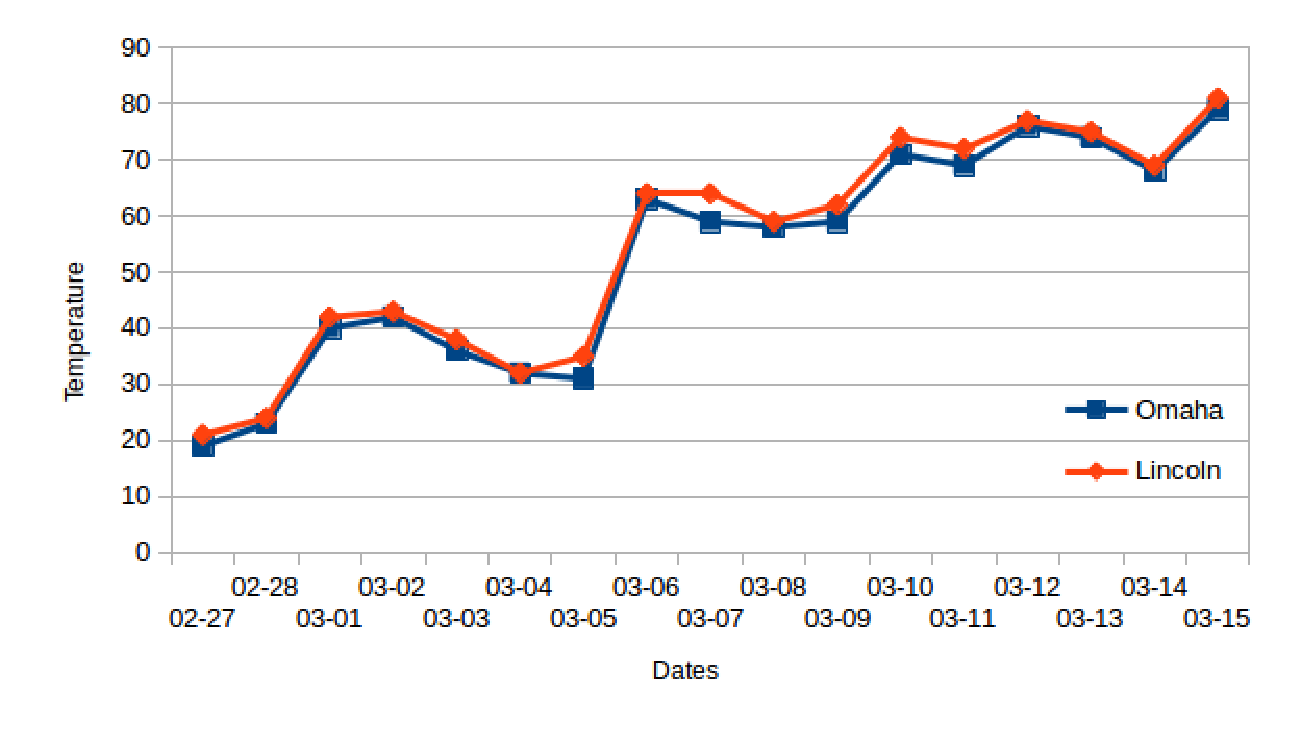
\includegraphics[width=1.0\linewidth]{chart1} \\
\mbox{\small{(a)}}\\
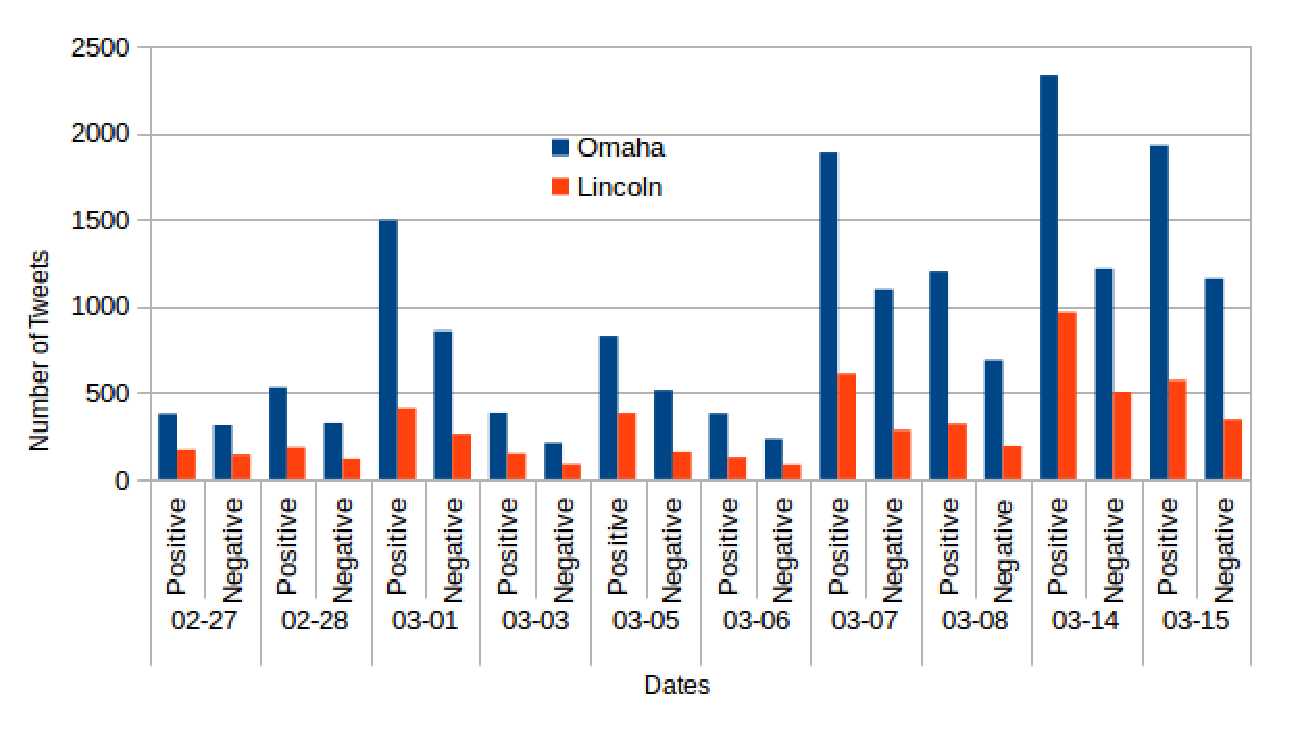
\includegraphics[width=1.0\linewidth]{chart2} \\
\mbox{\small{(b)}}\\
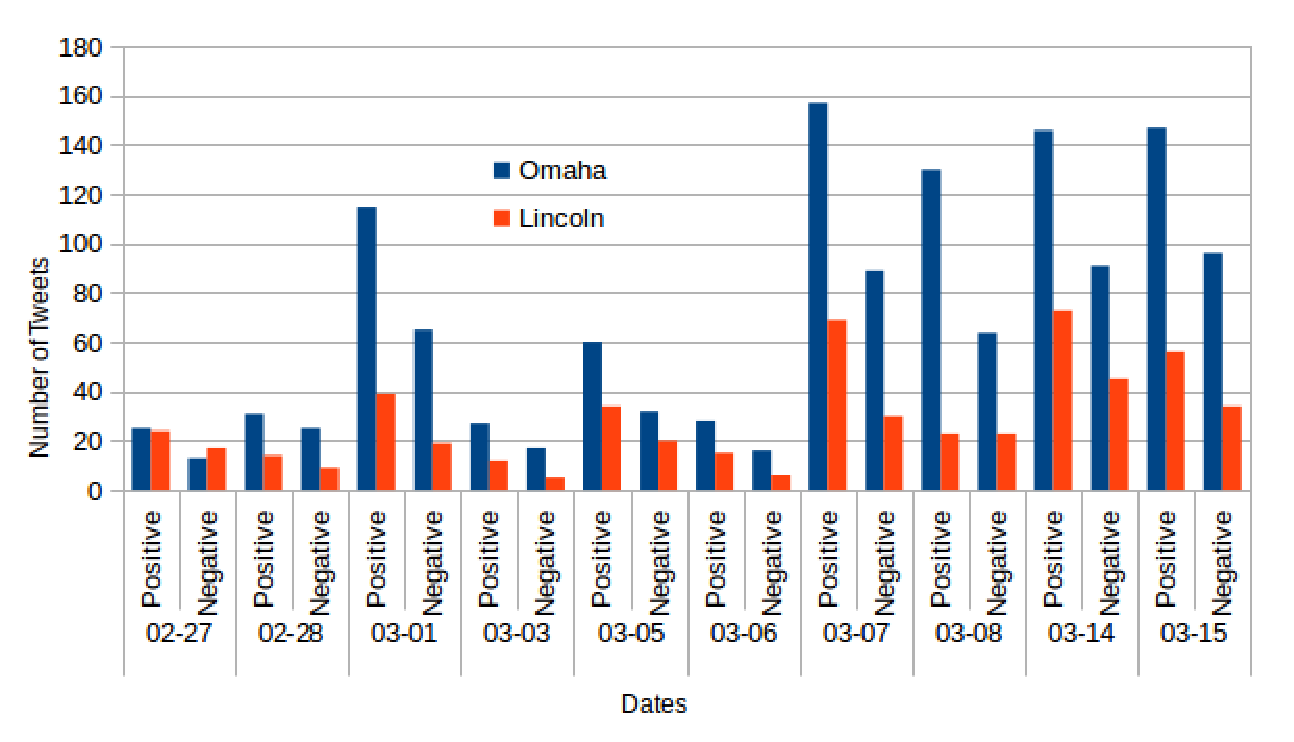
\includegraphics[width=1.0\linewidth]{chart3} \\
\mbox{\small{(c)}}
\end{center}
\vspace{-.1in}
\caption{The comparison of weather to sentiment.}
\label{fig:chart_1}
\end{figure}
%------------------------------------------------


In the first study, we use all collected tweets whether a tweet contains weather-related terms or not. Of all the cities, we see that Omaha and Lincoln have the most tweets, and thus we use these two cities to display our results. The weather patterns of the two weekends are shown in Figure~\ref{fig:chart_1}(a). Overall it shows a dramatically growing trend of temperature, roughly from $20^\circ$F to $80^\circ$F, as well as some fluctuations around the early March.

We choose to look at times where most of the population is awake (i.e., noon to 11 PM). From Figure~\ref{fig:chart_1}(b) we can see the tweets and their sentiment for select days through the two weeks, where more emphasis is placed on the first week and less on the later. Each date has a positive and negative count, where we clearly see a throughout pattern that the positive tweets outweigh the negative tweets. Another pattern that we see is that as the temperature increases the number of tweets increase. We also observe that more people tweet on Saturday than on Sunday. We think that this may be related to a number of factors: people go to church on Sunday where they choose to be among family, they do work around the house, or they do not have any eventful things which they feel they need to share.

We do not see that with the change of temperature that there is a clear trend of more positive tweets versus negative tweets. The number of positive tweets is at least half the amount of negative tweets. The only item that we could see which may be weather related is that the amount of negative tweets is percentage wise far more in the colder temperatures in comparison to the warmer temperatures. In lieu of not finding any clear results, we look at tweets only with words related to weather to see if we find any trends.


\subsubsection{Weather Related Tweets}

Other than using all the tweets we collected we filter the collected tweets for weather-related terms (i.e., snow, sunny, warm, cold, rain, etc.). We want to see if there is a stronger correlation in this situation compared to using all the tweets collected. In this situation, we are unfortunately limited to a few tweets. As shown in Figure \ref{fig:chart_1}(c), we see that the number of tweets drastically reduces to at most slightly less than 160 tweets for one day.

Fortunately, we are able to see a pattern with weather and positive tweets. There is a spike of tweets when there is warmer weather. This pattern is seen in both sets of tweet data sets. However, we are now able to confirm that the correlation is due to weather. As the weather increased slightly on March 1st we see a spike in amount of tweets overall (Figure \ref{fig:chart_1}(b)) and also when the tweets had weather-related words (Figure \ref{fig:chart_1}(c)). We can also see that in Figure \ref{fig:chart_1}(c) that with the warmer weather the number of tweets in relation to the weather increases by approximately twice the amount. We still see the trend of more positive tweets in comparison to negative tweets when using the filtered data set.


\subsection{Prediction}

Using the same data set we select a subset of two weekends to determine if the predicted value is close to the outcome. We choose March 6th, 7th and 8th for weekend one and March 13th, 14th and 15th for weekend two. The first weekend has between 10 to 20 degrees difference to the second weekend to take into account any change in weather patterns. We collect our predictions for Saturday and Sunday and compare them to the real sentiment of each hour. Again we focus on the two most populous cities in Nebraska: Lincoln and Omaha.

Figure~\ref{fig:predict} shows the accuracy of the three methods we used.

%------------------------------------------------
\begin{figure}[t]
\begin{center}
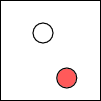
\includegraphics[width=1.0\linewidth]{sample}
\end{center}
\vspace{-.1in}
\caption{Accuracy of the different prediction methods.}
\label{fig:predict}
\end{figure}
%------------------------------------------------
